\documentclass{article}

\usepackage{a4wide}
\usepackage[utf8]{inputenc}
\usepackage[T1]{fontenc}
\usepackage[french]{babel}
\usepackage[babel=true]{csquotes} % guillemets français
\usepackage{graphicx}
\graphicspath{{Images/}}
\usepackage{color}
\usepackage{hyperref}
\hypersetup{colorlinks,linkcolor=,urlcolor=blue}

\usepackage{amsmath}
\usepackage{amssymb}


\title{\textbf{ Rapport - Developpement Mobile \\ Démineur}}
\author{Kamarouzamane Combo, Jeremie Legros\\
		L3 informatique\\
	  }
\date{\today}

\begin{document}

\maketitle % pour écrire le titre


%% Résumé:
\begin{abstract}
	Dans ce rapport, nous allons vous montrer ce que nous avons pu voir en développement mobile, et le projet que l'on a fait cette année.\\ 

	Notre projet porte sur le fameux jeu Démineur.\\
Règle du jeu: vous devez dévoiler toutes les cases sans jamais appuyer sur une bombe cachée.\\ Appuyez sur une case pour tenter de la dévoiler.\\ Vous pouvez également appuyer sur le bouton du drapeau, puis sur une case, afin de la marquer, si vous pensez qu\'une bombe se trouve à cet endroit.\\ Pour vous aider, les cases révélées indiqueront le nombres de bombes sur les 8 cases adjacentes.\\

	\textbf{Mots clés }: Android Studio, Xcode, Java, Swift, Activity
\end{abstract}


\section{Introduction}
\label{section:intro} % pour faire référence à la section ailleurs (\ref{...} voir plus bas)

	Actuellement, sur le marché du développement mobile, les deux principaux systèmes sont Android et iOS.~\cite{statOS}\\ Nous allons vous présenté notre jeu sur les deux systèmes Android et iOS, pour ce faire on a utilisé deux IDE pour les deux OS: Android Studio pour Android et Xcode pour iOS.   


\section{Description générale de l'application}
Voici une capture d'écran du Main Activity:
\begin{center}
  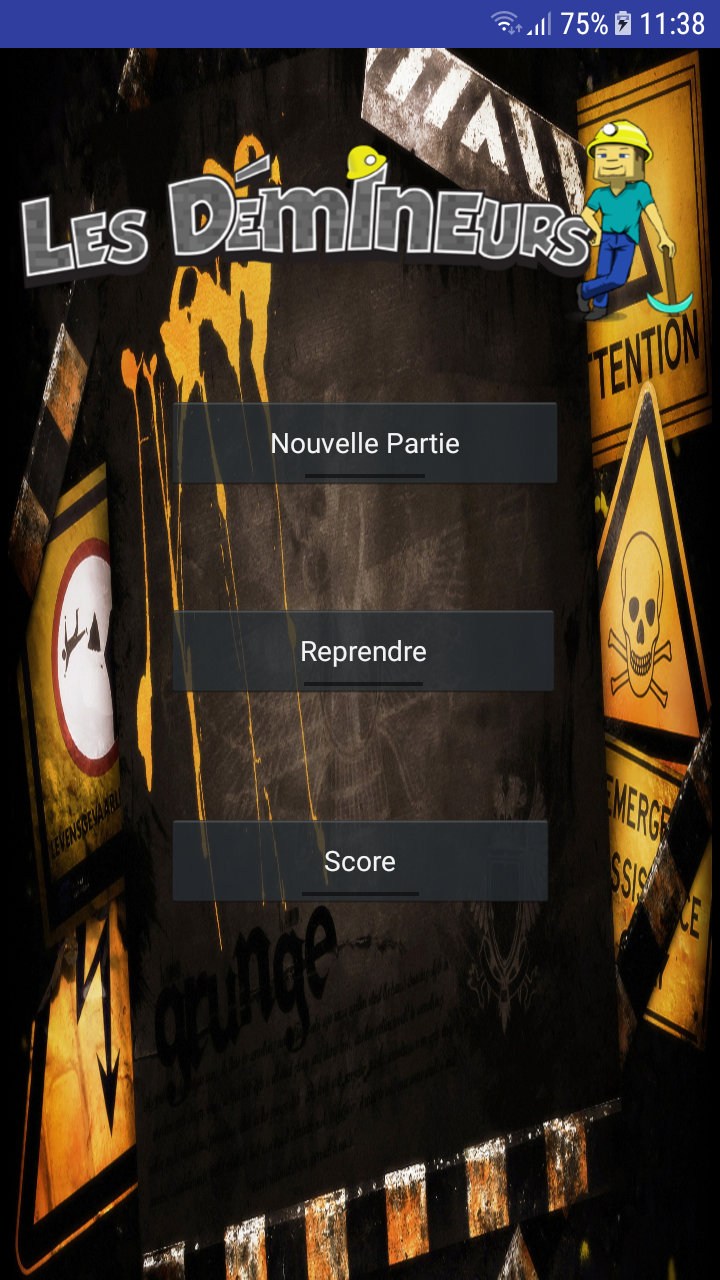
\includegraphics[scale=0.12]{Main.png}
\end{center}
	L' application fonctionne sur Android et iOS, elle fonctionne correctement sur 
tout type d' \'ecran (grand, petit, …), en mode portrait et paysage.\\

Mais que fait-elle exactement ? \\
	C'est le jeu Démineur :  But est de dévoiler toutes les cases sans jamais appuyer sur une bombe cachée.\\
	Au lancement de l’ application, la page d’ accueil apparaître et donner la
possibilité à l' utilisateur de jouer une nouvelle partie (choix : le niveau de difficulté), de reprendre une partie sauvegardée ou de consulter la liste des scores enregistrés.



\begin{itemize}
\item la documentation d'\textit{Android}~\cite{androidDoc}
  est bien écrite,
\item celle d'\textit{iOS}~\cite{iosDoc} aussi!
\end{itemize}
% \cite{...} permet de faire référence à des éléments de la
% bibliographie.

Une liste numérotée:
\begin{enumerate}
\item premier item
\item second item
\end{enumerate}



\section{Architecture du code}
% \ref{...} permet de faire référence à un élément défini
% ailleurs dans le document (voir \label{...} plus haut).
Contrairement à la section~\ref{section:intro},
moi je dis: \textit{Coucou!}

\subsection{Android} %% une sous-section
Pour écrire du code, on peut par exemple utiliser l'environnement
\textit{verbatim}:
\begin{verbatim}
public class Main {
   public static void main(String[] args) {
      System.out.println("Hello World!");
   }
}
\end{verbatim}

\subsection{iOS} %% une autre sous-section


\section{Quelques points délicats/intéressants}


\section{Conclusion générale}
	Ce cours était bien utile, notamment en ce qui concerne la création d'application mobile.


%%% La bibliographie:
\bibliographystyle{plain}
\bibliography{ma_biblio}

\end{document}
